% Switching cell: Vdc -- [D parallel with L] -- Q (IGBT) -- GND
% D internal right branch; L external parallel branch on right
% Gate drive: Vg through Rg to IGBT gate, with ig current label

\documentclass[border=5pt]{standalone}
\usepackage{tikz}
\usepackage[american,cuteinductors,smartlabels]{circuitikz}

\ctikzset{bipoles/thickness=0.7}
\ctikzset{bipoles/length=1.5cm}
\ctikzset{bipoles/resistor/width=0.7}
\ctikzset{bipoles/resistor/height=0.25}
\ctikzset{bipoles/diode/height=0.3}
\ctikzset{bipoles/diode/width=0.3}
\ctikzset{tripoles/thickness=0.7}
\ctikzset{bipoles/battery1/height=0.7}

\tikzstyle{every node}=[font=\Large]
\tikzstyle{every path}=[line width=0.9pt, line cap=round, line join=round]

\begin{document}
\begin{circuitikz}

  \coordinate (VBottom) at (0,0);

  %--- Input voltage source Vdc (+ at top via invert, consistent with reference style)
  \draw (VBottom) to[battery1, l=$V_{dc}$, invert] ++(0,6) coordinate (VTop);

  %--- Top horizontal rail
  \draw (VTop) to[short] ++(5,0) coordinate (TopRight);

  %--- Diode D: spans full 2.5 units to align visually with inductor L (also 2.5 units)
  %    invert = cathode at top, anode at bottom (freewheeling direction)
  \draw (TopRight) to[D*, l=$D$, invert] ++(0,-2.5) coordinate (DNode);

  %--- Inductor L: external parallel branch, right of main rectangle
  %    3-unit gap; (LTop|-DNode) auto-spans full height to match DNode level
  %    i>^= puts iL label on LEFT side, l_= keeps L label on RIGHT → no clutter
  \draw (TopRight) to[short] ++(3,0) coordinate (LTop);
  \draw (LTop) to[L, l_=$L$, i>^=$i_L$] (LTop|-DNode) coordinate (LBot);
  \draw (LBot) -- (DNode);

  %--- IGBT Q: vertical orientation, collector (C) anchored at DNode
  \draw (DNode) to[short] ++(0,-0.5)
    node[nigbt, anchor=C,
         label={[xshift=0.5cm, yshift=0] \normalsize $Q$}] (Q1) {};

  %--- IGBT emitter (E) drops straight to bottom rail
  \draw (Q1.E) -- (Q1.E|-VBottom) coordinate (QGnd);

  %--- Close the main power loop: bottom rail
  \draw (QGnd) -- (VBottom);

  %--- Gate drive circuit
  %    Q1.B = gate terminal (extends left from IGBT body)
  %    i<_ = current arrow pointing RIGHT (into gate, against the leftward draw direction)
  \draw (Q1.B) to[short, i<_=$i_g$] ++(-1.5,0) coordinate (GateLeft)
    to[R, l=$R_g$] ++(-1.5,0) coordinate (VgTop);

  %--- Gate voltage source Vg: drawn upward from ground to VgTop
  %    invert = + at top (VgTop side) = drives gate positive w.r.t. source
  %    consistent with Boost.tex: upward source + invert = + at top
  \draw (VgTop|-VBottom) to[V, l=$V_g$, invert] (VgTop);

  %--- Connect Vg ground terminal to main bottom rail
  \draw (VgTop|-VBottom) -- (VBottom);

\end{circuitikz}

% --- Gate drive timing diagram: double pulse pattern
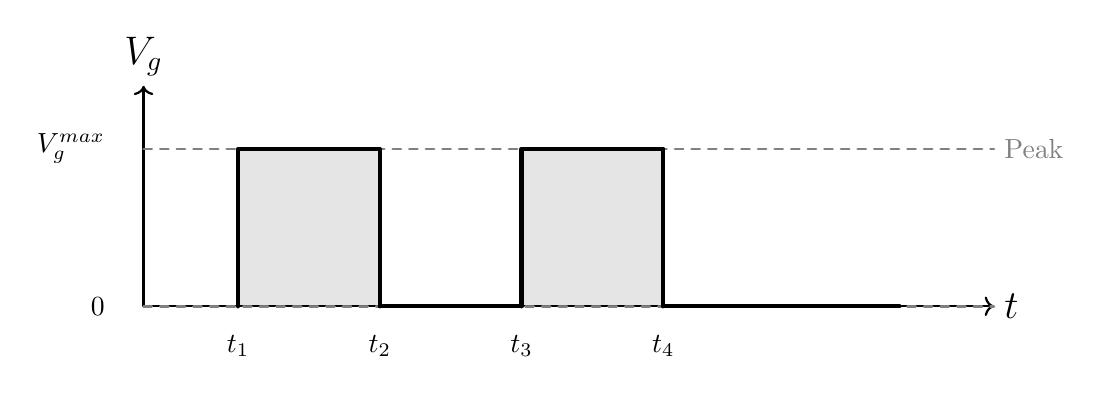
\begin{tikzpicture}[xscale=1.2, yscale=0.8]
  % Axes
  \draw[thick, ->] (0,0) -- (9,0) node[right, font=\Large] {$t$};
  \draw[thick, ->] (0,0) -- (0,3.5) node[above, font=\Large] {$V_g$};

  % Voltage reference lines
  \draw[gray, dashed] (0,2.5) -- (9,2.5) node[right, font=\normalsize, gray] {Peak};
  \draw[gray, dashed] (0,0) -- (9,0);

  % First pulse: t=1 to t=2.5
  \draw[line width=1.5pt] (1,0) -- (1,2.5) -- (2.5,2.5) -- (2.5,0);
  \fill[black, opacity=0.1] (1,0) -- (1,2.5) -- (2.5,2.5) -- (2.5,0);

  % Dead time (low)
  \draw[line width=1.5pt] (2.5,0) -- (4,0);

  % Second pulse: t=4 to t=5.5
  \draw[line width=1.5pt] (4,0) -- (4,2.5) -- (5.5,2.5) -- (5.5,0);
  \fill[black, opacity=0.1] (4,0) -- (4,2.5) -- (5.5,2.5) -- (5.5,0);

  % Trailing edge
  \draw[line width=1.5pt] (5.5,0) -- (8,0);

  % Time labels
  \node[below, font=\normalsize] at (1,-.3) {$t_1$};
  \node[below, font=\normalsize] at (2.5,-.3) {$t_2$};
  \node[below, font=\normalsize] at (4,-.3) {$t_3$};
  \node[below, font=\normalsize] at (5.5,-.3) {$t_4$};

  % Voltage label
  \node[left, font=\normalsize] at (-.3,2.5) {$V_g^{max}$};
  \node[left, font=\normalsize] at (-.3,0) {$0$};
\end{tikzpicture}

\end{document}
